\section{Risultati sperimentali}
\label{sec:risultati}

I dati sperimentali sono stati raccolti utilizzando tre macchine:
\begin{itemize}
    \item \textbf{Macchina A}: \textbf{Intel Core i7-8750H} (8$^\text{a}$ gen, 6 core, 12 thread, fino a 4{,}1~GHz), \textbf{16~GB di RAM DDR4}, SSD \textbf{SanDisk 128~GB SATA M.2} (\texttt{SD9SN8W128G1002}), sistema operativo \textbf{Arch Linux}, kernel \texttt{6.15.6}, file system \texttt{btrfs}.
    \item \textbf{Macchina B}: \textbf{Intel Core i7-12700H} (12$^\text{a}$ gen, 14 core, 20 thread, fino a 4{,}7~GHz), \textbf{16~GB di RAM DDR4}, SSD \textbf{NVMe PCIe da 1~TB} (\texttt{MTFDKBA1T0TFH-1BC1AABHA}), sistema operativo \textbf{Ubuntu 22.04}, kernel \texttt{6.12.10}, file system \texttt{ext4}.
    \item \textbf{Macchina C}: \textbf{Intel Core i5-12450H} (12$^\text{a}$ gen, 8 core, 12 thread, fino a 4{,}4~GHz), \textbf{16~GB di RAM DDR4}, SSD \textbf{NVMe PCIe da 512~GB} (modello generico \texttt{PCIe-8 SSD 512GB}), sistema operativo \textbf{Arch Linux}, kernel \texttt{6.15.6}, file system \texttt{xfs}.
\end{itemize}

Le macchine erano collegate tramite una rete Ethernet gigabit, con una latenza di circa 0{,}3~ms.
Erano configurate con lo scaling della frequenza, il turbo boost e l'hyper-threading disabilitati, al fine di garantire prestazioni costanti e ridurre la variabilità dei risultati.

I grafici mostrano la latenza osservata al variare della frequenza delle operazioni, per diversi percentili (dal P0 al P100).
Ciascun test è stato eseguito per un periodo di 20~secondi, con una frequenza crescente a partire da 1000~Hz fino al cedimento del sistema.

\subsection{Operazione \texttt{set}}
\label{subsec:risultati-set}

\begin{figure}[htbp]
    \centering
    \begin{minipage}[t]{0.48\textwidth}
        \centering
        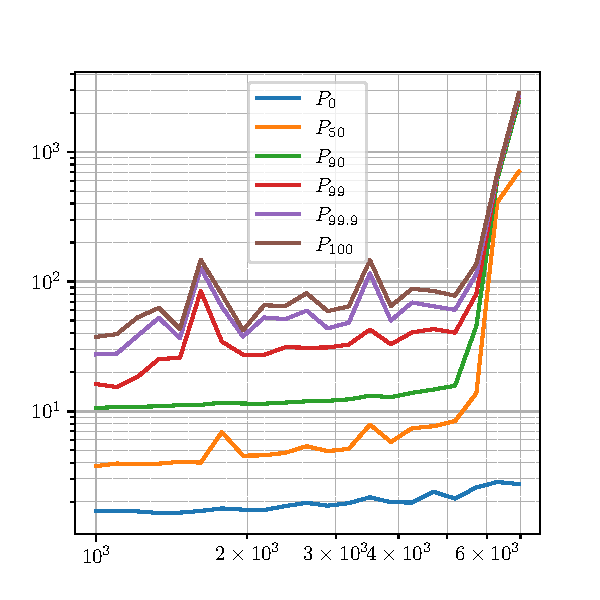
\includegraphics[width=\textwidth]{03-risultati/bench-set-a}
        \caption*{Macchina A}
    \end{minipage}
    \hfill
    \begin{minipage}[t]{0.48\textwidth}
        \centering
        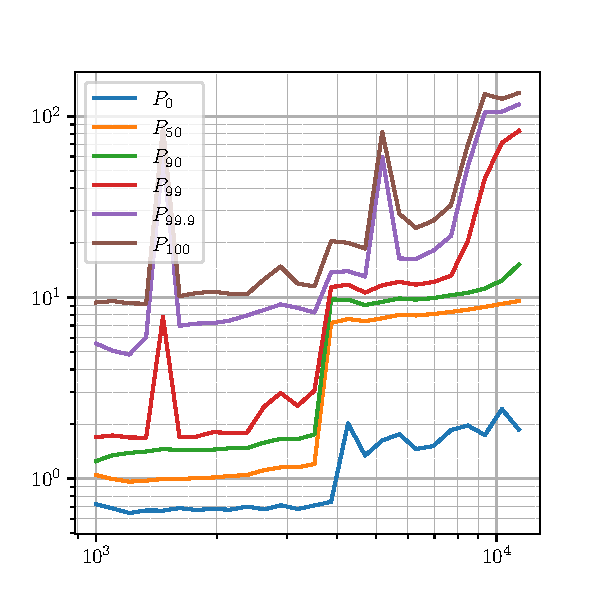
\includegraphics[width=\textwidth]{03-risultati/bench-set-c}
        \caption*{Macchina B}
    \end{minipage}

    \vspace{0.5cm}
    \begin{minipage}[t]{0.48\textwidth}
        \centering
        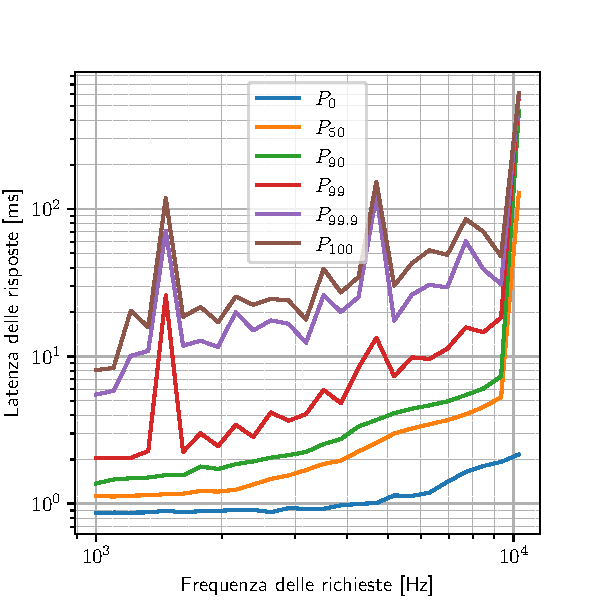
\includegraphics[width=\textwidth]{03-risultati/bench-set-h}
        \caption*{Macchina C}
    \end{minipage}

    \caption{Prestazioni delle macchine in scrittura. Ogni grafico mostra, al variare della frequenza delle operazioni [Hz], la latenza [ms] osservata per diversi percentili (dal P0 al P100).}
    \label{fig:bench-set}
\end{figure}

\begin{figure}[htbp]
    \centering
    \begin{minipage}[t]{0.48\textwidth}
        \centering
        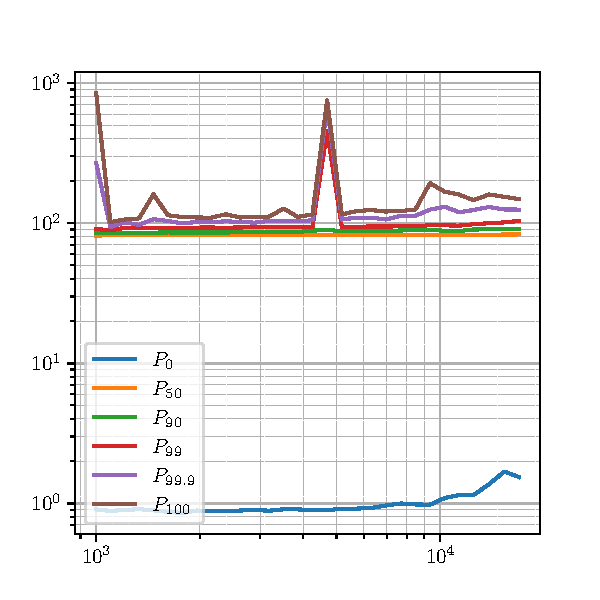
\includegraphics[width=\textwidth]{03-risultati/bench-set-all}
        \caption*{Chiavi distribuite uniformemente sulle tre macchine}
    \end{minipage}
    \hfill
    \begin{minipage}[t]{0.48\textwidth}
        \centering
        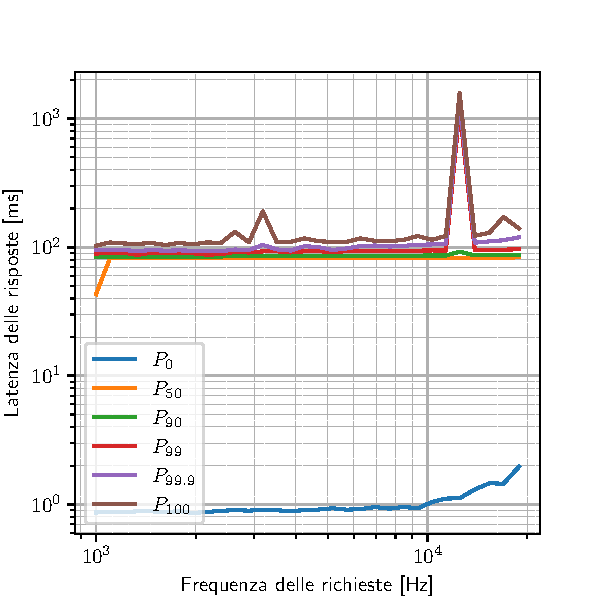
\includegraphics[width=\textwidth]{03-risultati/bench-set-all-balance}
        \caption*{Chiavi distribuite sulle tre macchine con pesi bilanciati $6{:}10{:}10$}
    \end{minipage}

    \caption{Prestazioni delle macchine in scrittura distribuita. Ogni grafico mostra, al variare della frequenza delle operazioni [Hz], la latenza [ms] osservata per diversi percentili (dal P0 al P100).}
    \label{fig:bench-set-all}
\end{figure}

In figura~\ref{fig:bench-set} sono riportati i risultati ottenuti dalle tre macchine durante le operazioni di scrittura (\texttt{set}).
Durante i test, la limitazione del throughput era disabilitata, permettendo di osservare le prestazioni massime raggiungibili da ciascuna macchina.
I grafici mostrano che le macchine A, B e C hanno raggiunto, rispettivamente, un throughput massimo di $6{,}9\,{\times}\,10^3$, $11{,}3\,{\times}\,10^3$ e $10{,}3\,{\times}\,10^3$ operazioni al secondo.

In figura~\ref{fig:bench-set-all} sono presentati i risultati ottenuti mediante l'utilizzo congiunto delle tre macchine, con chiavi distribuite tra esse senza replicazione (parametri $n=1, r=1, w=1$).
Distribuendo le chiavi in modo uniforme (con $b_i$ tutti uguali), è stato raggiunto un throughput complessivo di $16{,}9\,{\times}\,10^3$ operazioni al secondo.
Utilizzando invece una distribuzione pesata delle chiavi, con pesi pari a $6{:}10{:}10$, il throughput complessivo è salito a $18{,}8\,{\times}\,10^3$ operazioni al secondo, dimostrando l'importanza del meccanismo di allocazione della banda per ottimizzare le prestazioni in scenari eterogenei.
Sebbene la somma delle capacità individuali sia pari a $28{,}6\,{\times}\,10^3$ operazioni al secondo, il valore effettivamente osservato risulta inferiore.
Si osserva inoltre un incremento della latenza rispetto all'esecuzione su una singola macchina; tuttavia, a differenza dei test singoli, la latenza rimane pressoché costante all'aumentare della frequenza delle operazioni.
Si ipotizza che tali effetti siano attribuibili all'overhead introdotto dalla comunicazione e dal coordinamento tra i nodi distribuiti.

\subsection{Operazione \texttt{get}}
\label{subsec:risultati-get}

\begin{figure}[htbp]
    \centering
    \begin{minipage}[t]{0.48\textwidth}
        \centering
        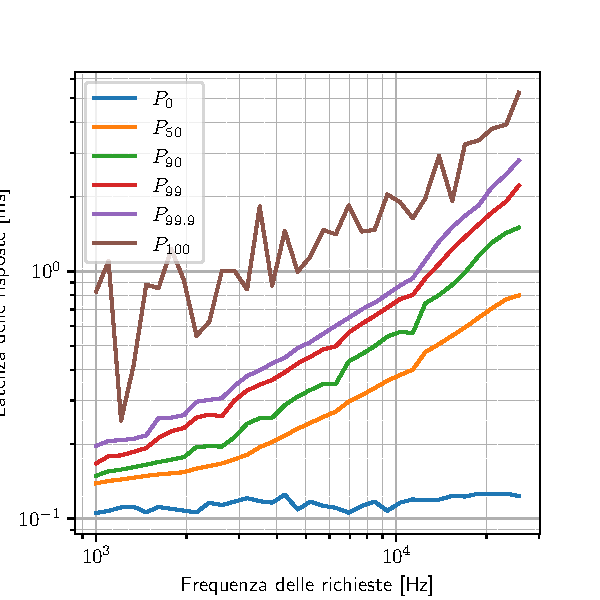
\includegraphics[width=\textwidth]{03-risultati/bench-get-a}
        \caption*{Macchina A}
    \end{minipage}
    \hfill
    \begin{minipage}[t]{0.48\textwidth}
        \centering
        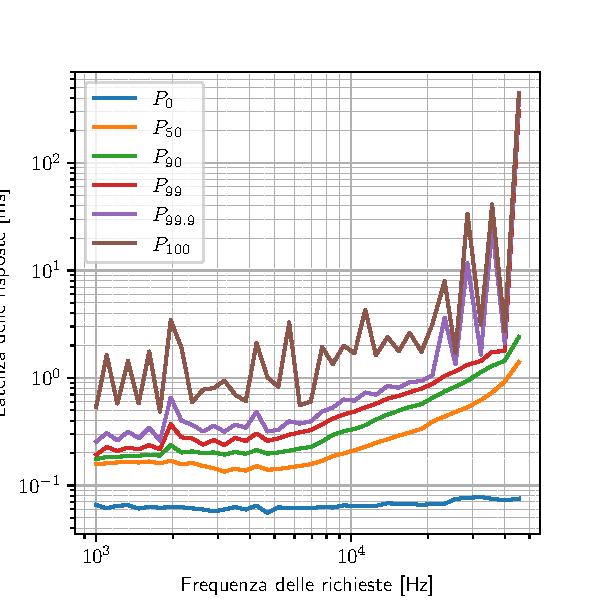
\includegraphics[width=\textwidth]{03-risultati/bench-get-c}
        \caption*{Macchina B}
    \end{minipage}

    \vspace{0.5cm}
    \begin{minipage}[t]{0.48\textwidth}
        \centering
        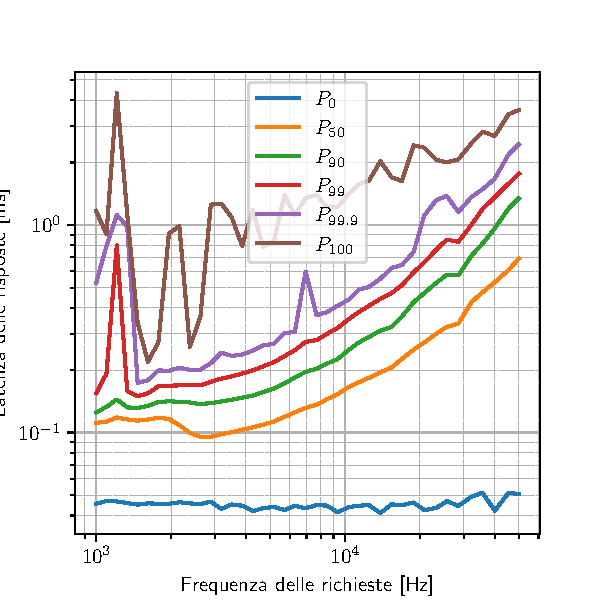
\includegraphics[width=\textwidth]{03-risultati/bench-get-h}
        \caption*{Macchina C}
    \end{minipage}
    \hfill
    \begin{minipage}[t]{0.48\textwidth}
        \centering
        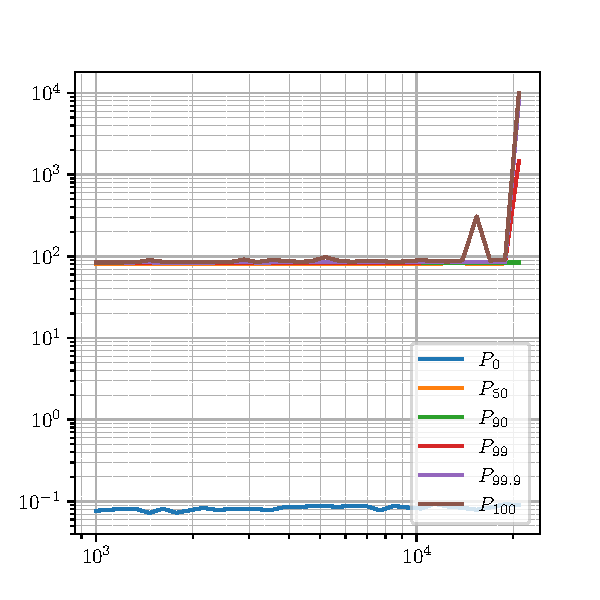
\includegraphics[width=\textwidth]{03-risultati/bench-get-all}
        \caption*{Chiavi distribuite uniformemente sulle tre macchine}
    \end{minipage}

    \caption{Prestazioni delle macchine in lettura. Ogni grafico mostra, al variare della frequenza delle operazioni [Hz], la latenza [ms] osservata per diversi percentili (dal P0 al P100).}
    \label{fig:bench-get}
\end{figure}

In figura~\ref{fig:bench-get} sono riportati i risultati ottenuti dalle tre macchine durante le operazioni di lettura (\texttt{get}).
Anche in questo caso, la limitazione del throughput era disabilitata, consentendo di osservare le prestazioni massime.
Le macchine A, B e C hanno raggiunto, rispettivamente, un throughput massimo di $25{,}6\,{\times}\,10^3$, $45{,}4\,{\times}\,10^3$ e $50{,}0\,{\times}\,10^3$ operazioni al secondo.

Mediante l'utilizzo congiunto delle tre macchine, con chiavi distribuite uniformemente tra di esse e senza replicazione ($n=1, r=1, w=1$), è stato raggiunto un throughput complessivo di $20{,}8\,{\times}\,10^3$ operazioni al secondo, inferiore rispetto a quello delle singole macchine.
Il costo di una lettura da disco è molto inferiore rispetto a quello di una scrittura, grazie alla presenza della cache del file system.
Questo evidenzia l'overhead della comunicazione tra macchine, che incide negativamente sulle prestazioni complessive.
Si ipotizza che, utilizzando un database di dimensioni superiori alla RAM disponibile (e quindi riducendo l'efficacia della cache), l'utilizzo di più macchine possa tornare vantaggioso.
Tuttavia, non è stato possibile verificare direttamente questa ipotesi.

\subsection{Multitenant}
\label{subsec:risultati-multitenant}

\begin{figure}[htbp]
    \centering
    \begin{minipage}[t]{0.48\textwidth}
        \centering
        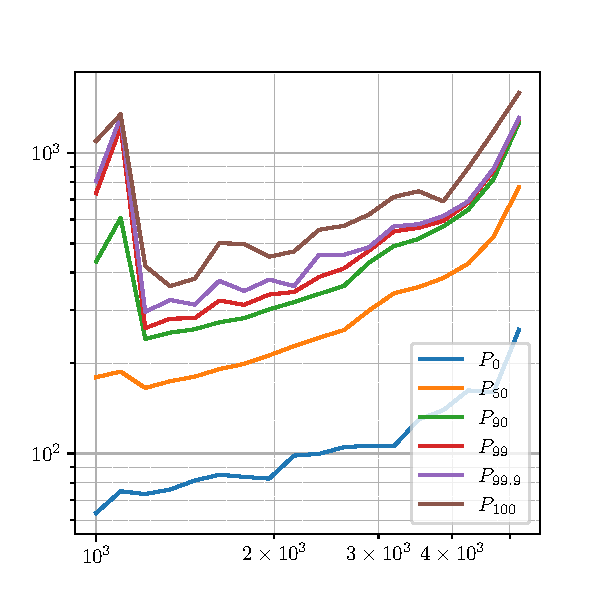
\includegraphics[width=\textwidth]{03-risultati/bench-set-no-throttling}
        \caption*{Senza limitazione del throughput}
    \end{minipage}
    \hfill
    \begin{minipage}[t]{0.48\textwidth}
        \centering
        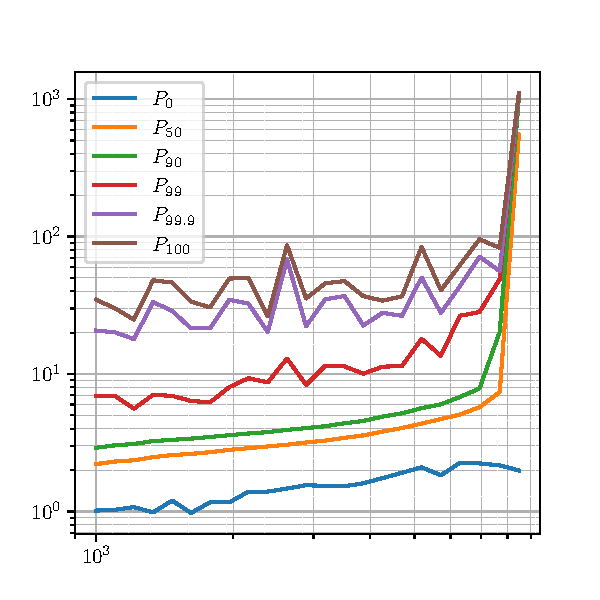
\includegraphics[width=\textwidth]{03-risultati/bench-set-throttling}
        \caption*{Con limitazione del throughput}
    \end{minipage}

    \caption{Prestazioni della macchina in scrittura, con e senza limitazione del throughput, in presenza di client malevoli. Ogni grafico mostra, al variare della frequenza delle operazioni [Hz], la latenza [ms] osservata per diversi percentili (dal P0 al P100).}
    \label{fig:bench-throttling}
\end{figure}

In figura~\ref{fig:bench-throttling} sono riportati i risultati ottenuti dalla macchina C durante operazioni di scrittura in un contesto multitenant.
Durante il test erano presenti due tabelle, X e Y, con bande rispettive di 8000 e 1000 operazioni al secondo, e un client malevolo che cercava di saturare le risorse scrivendo sulla tabella Y.
Il client malevolo era composto da due parti:
\begin{itemize}
    \item Una componente che lancia 1000 task, ognuno dei quali esegue scritture continue sulla tabella Y, mantenendo quindi sempre 1000 operazioni simultanee in corso.
    \item Una componente che genera 4000 operazioni al secondo in modalità asincrona, attendendo in background il completamento di ciascuna richiesta senza bloccare il thread principale.
\end{itemize}

I grafici mostrano le prestazioni osservate per la tabella X, sia in presenza che in assenza della limitazione del throughput (vedi sezione~\ref{subsec:limitazione-throughput}).
In assenza di tale limitazione, la latenza al $50^\circ$ percentile parte da circa 180~ms e il throughput massimo raggiunto è pari a $5{,}2\,{\times}\,10^3$ operazioni al secondo, un valore inferiore rispetto a quello che dovrebbe essere garantito.
Con la limitazione del throughput attiva, invece, la latenza al $50^\circ$ percentile rimane sotto i 10~ms fino al raggiungimento del throughput massimo garantito di 8000 operazioni al secondo.
